\documentclass[10pt,a5paper]{article}
\usepackage[utf8]{inputenc}
\usepackage[english,russian]{babel}
\usepackage[OT1]{fontenc}
\usepackage{amsmath}
\unitlength=1mm
\usepackage{amsfonts}
\usepackage{amssymb}
\usepackage[left=1.2 cm,right=1.2 cm,top=1.8 cm,bottom=1.8 cm]{geometry}
\usepackage{graphicx}
\graphicspath{img/}
\title{Астрадь}
\begin{document}

\begin{titlepage}
	
	\begin{center}
	\vspace*{5 cm}
		{\Huge \bfseries \scshape Астрадь}
	\end{center}
\end{titlepage}

\tableofcontents
\newpage

\section{Элементы небесной механики}

\subsection{Закон всемирного тяготения}

Сила притяжения между двумя телами с массами M и m, где $G\approx\ 6.67\cdot \cdot10^{-11}\frac{\text{Н}\cdot \text{м}^2}{\text{кг}^2}$ --- гравитационная постоянная.$$F=G\frac{Mm}{R^2}$$
Потенциал точечной (или сферически симметричной) массы $M$ в точке $r$; он равен энергии единичной массы, принесенной из бесконечности в эту точку.$$U=-\frac{GM}{r}$$
Ускорение свободного падения.$$g=G\frac{M}{R^2}$$
Ускорение свободного падения для тел солнечной системы:
\begin{table}[h!]
\centering
\begin{tabular}{|c|c|c|c|}
\hline 
\textbf{Планета} & $\mathbf{g}$, \textbf{м/c$~^2$} & \textbf{Планета} & $\mathbf{g}$, \textbf{м/c$~^2$}\\
\hline
Солнце & 274 & Марс & 3,7\\
\hline
Меркурий & 3,7 & Юпитер & 24,8\\
\hline
Венера & 8,9 & Сатурн & 10,4\\
\hline
Земля & 9,8 & Уран & 8,8\\
\hline
Луна & 1,6 & Нептун & 11,2\\
\hline
\end{tabular}
\end{table}
\subsection{Закон сохранения энергии и типы орбит}

Закон сохранения энергии. $E_0$ - константа, равна сумме кинетической и потенциальной энергии единичной массы.$$\frac{v^2}{2}-\frac{GM}{r}=E_0$$

Если $E_0>0$, то траектория тела --- гипербола, ветви которой асимптотически приближаются к двум прямым.

Если $E_0=0$, то траектория тела --- гипербола. При параболической и гиперболический траекториях движение не ограничено.

Если $E_0<0$, то траектория тела --- эллипс. При эллиптической траектории движение ограничено.

Параболическая скорость - минимальная скорость, при которорй тело покидает центральную массу$M$.$$V_p=\sqrt{\frac{2GM}{r}}$$

На рис. 1 представлены примеры возможных траекторий тела относительно центрального (точка C).

При $v_0>v_p$ (пароболическая скорость) --- тело движется по гиперболе,при $v_0=v_p$ --- тело движется по пораболе, а при $v_0<v_p$ --- по эллипсу.
\begin{center}
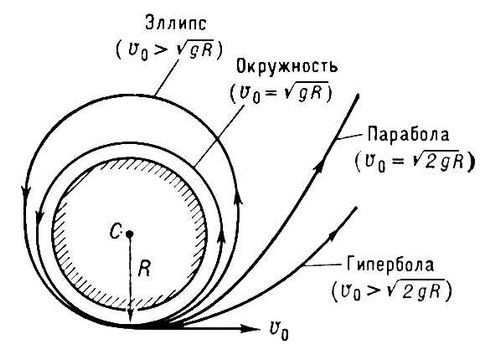
\includegraphics[scale=0.35]{i010-001-245539763.jpg}
\begin{figure}[h!]
\caption{ Возможные траектории тела}
\end{figure}
\end{center}
\subsection{Законы Кеплера}

\bfseries 1 закон: \mdseries  Все планеты движутся по эллиптическим орбитам, в одном из которых находится Солнце.(Рис. 2)
\begin{center}
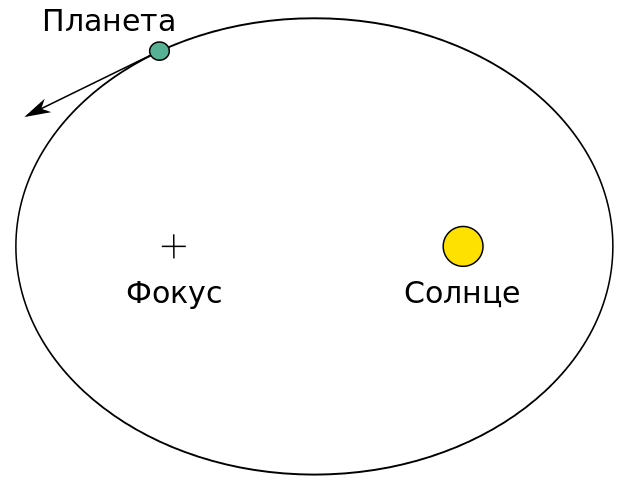
\includegraphics[scale=0.2]{picture-081-314}
\begin{figure}[h!]
\caption {Первый закон Кеплера}
\end{figure}
\end{center}

\bfseries 2 закон: \mdseries Радиус-вектор планеты описывает за равные промежутки времени равные площади.(Рис. 3)
\begin{center}
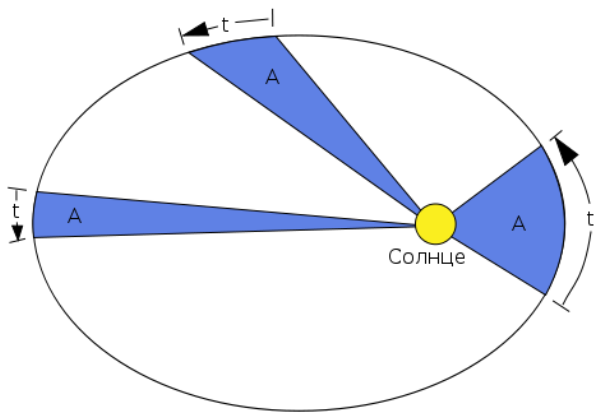
\includegraphics[scale=0.4]{32}
\begin{figure}[h!]
\caption {Второй закон кеплера}
\end{figure}
\end{center}$$\frac{dS}{dt}=const$$
\bfseries 3 закон: \mdseries Квадраты периодов обращения планет относятся, как кубы больших полуосей их орбит.
$$\frac{T^2_1}{T^2_2}=\frac{a^3_1}{a^3_2}$$
Где $a$ --- большая полуось, $T$ --- период обращения.
Обобщённый Ньютоном 3 закон имеет слейдующий вид:
$$\frac{T^2_1(M+m_1)}{T^2_2(M+m_2)}=\frac{a^3_1}{a^3_2} \text{ или } \frac{T^2}{a^3}=\frac{4\pi^2}{G(M+m)}$$
Где $M$ --- масса центрального тела, $m_1$ и $m_2$ --- массы обращающихся тел. Так как массы планет m много меньше массы звезды $M$, то $M+m\approx M$
\subsection{Первая, вторая и третья космические скорости} 

\bfseries Первая космическая скорость \mdseries --- минимальная скорость, необходимая для того, чтобы маломассивное тело стало искусственным спутником центрального тела.
$$v_1=\sqrt{\frac{GM}{R}}$$
Где $M$ --- масса массивного тела.

\bfseries Вторая космическая скорость \mdseries --- минимальная скорость, необходимая для того, чтобы маломассивное тело преодолело гравитационное притяжение центрального тела и покинуло замкнутую орбиту вокруг последнего. 
$$v_2=v_p=\sqrt{2gR}=\sqrt{\frac{2GM}{R}}=\sqrt{2}v_1$$
$v_1$ и $v_2$ на некоторых телах Солнечной системы:
\begin{table}[h!]
\centering
\begin{tabular}{|c|c|c|}
\hline
\textbf{Планета} & $\mathbf{v_1}$,\textbf{км/c} & $\mathbf{v_2}$,\textbf{км/c}\\
\hline
Солнце & 436,8 & 617,7\\
\hline
Меркурий & 3,0 & 4,3\\
\hline
Венера & 7,4 & 10,5\\
\hline
Земля & 7,9 & 11,2\\
\hline
Луна & 1,7 & 2,4\\
\hline
Марс & 3,5 & 5,0\\
\hline
Юпитер & 42,0 & 59,5\\
\hline
Сатурн & 25,1 & 35,5\\
\hline
Уран & 15,0 & 21,3\\
\hline
Нептун & 16,6 & 23,5\\
\hline
\end{tabular}
\end{table}

Скорость искусственного небесного тела на высоте $h$.$$v_h=\sqrt{\frac{GМ}{R+h}}=\sqrt{\frac{gR^2}{R+h}}$$

\bfseries Третья космическая скорость \mdseries --- минимальная скорость, которую необходимо придать находящемуся вблизи поверхности Земли телу, что-бы оно могло преодолеть гравитационное притяжение Земли и Солнца и покинуть пределы Солнечной системы.
$$v_3=\sqrt{(\sqrt{2}-1)^2v^2_1+v^2_2}$$ 
\subsection{Движение по эллиптической орбите}

(Численно) Для тел солнечной системы.$$T^2_{\text{год}}=a^3_{\text{а.е.}}$$
Средняя скорость планет Солнечной системы.$$v_{\text{орб}}=\sqrt{\frac{GM}{a}}\approx \frac{29,8}{\sqrt{a}}$$
Скорость в апоцентре, $e$ --- эксцентриситет.$$v_{\text{аф}}=v_{\text{орб}}\sqrt{\frac{1-e}{1+e}}$$
Скорость в перицентре, $e$ --- эксцентриситет.$$v_{\text{пер}}=v_{\text{орб}}\sqrt{\frac{1+e}{1-e}}$$
Скорость в точке орбиты, удалённой на расстояние $r$ от центрального тела, $M$ --- масса центрального тела.$$v=\sqrt{GM\left(\frac2r - \frac1a\right)}$$
Скорость в точке орбиты, для которой истинная аномалия $\nu$, $p$ --- фокальный параметр.$$v=\sqrt{\frac{GM}{p}\cdot(1+2e\nu+e^2)}$$
\subsection{Синодический период}

\textbf{Синодический период} --- промежуток времени между двумя последовательными одноимёнными конфигурациями планеты или Луны. Для Луны можно ввести другое определение --- промежуток времени между двумя последовательными одинаковыми фазами.

$S$ --- синодический период.

$T$ --- сидерический период.

$E$ --- сидерический период обращения Земли.

Для внешних планет:
$$\frac1S=\frac1E-\frac1T$$
Для внутренних планет:
$$\frac1S=\frac1T-\frac1E$$

В случае, если тело обращается по орбите в протвоположную сторону, то связь между синодическим и сидерическим периодами тела выглядит так:
$$\frac1S=\frac1E+\frac1T$$
\subsection{Конфигурации планет}
\begin{center}
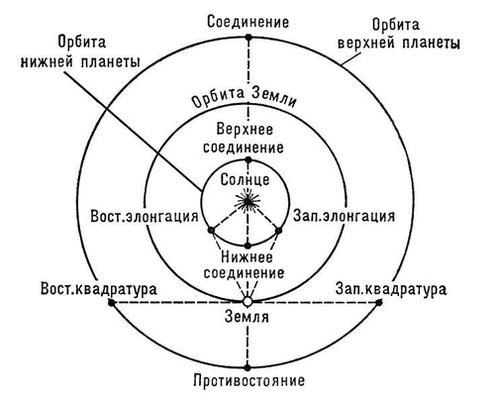
\includegraphics[scale=0.571]{468_1}
\begin{figure}[h!]
\caption{Конфигурации планет}
\end{figure}
\end{center}
\subsection{Кеплеровы элементы орбиты}

\textbf{Кеплеровы элементы} --- шесть элементов орбиты, определяющие положение небесного тела в пространстве в задаче двух тел:
\begin{enumerate}
\item Большая полулось($a$);
\item Эксцентриситет ($e$);
\item Наклонение($i$);
\item Аргумент перицентра($\omega$);
\item Долгота восходящего узла($\Omega$);
\item Средняя аномалия ($M_0$);
\end{enumerate}
Первые два определяют форму орбиты, третий, четвёртый и пятый — ориентацию плоскости орбиты по отношению к базовой системе координат, шестой — положение тела на орбите (Рис.5).

\textbf{Наклонение} --- небесного тела — это угол между плоскостью его орбиты и плоскостью эклиптики.
\textbf{Аргумент перицентра} --- угол между направлениями из притягивающего центра на восходящий узел орбиты и на перицентр.

\textbf{Долгота восходящего узла} --- угол в плоскости эклиптики между направлением на точку весеннего равноденствия и восходящий узел орбиты. Отсчитывается против часовой стрелки от направления на точку весеннего равноденствия.

\textbf{Средняя аномалия} для тела, движущегося по невозмущённой орбите --- произведение его среднего движения и интервала времени после прохождения перицентра.

\textbf{Узлы орбиты} --- точки пересечения орбиты и плоскости эклиптики.

\textbf{Восходящий узел} --- точка, в которой тело пересекает плоскость эклиптики при движении в северноим направлении, а \textbf{нисходящий} --- в южном.

\textbf{Истинная аномалия ($\nu$)} --- угол между радиус вектором и направлением на перицентр.
\begin{center}
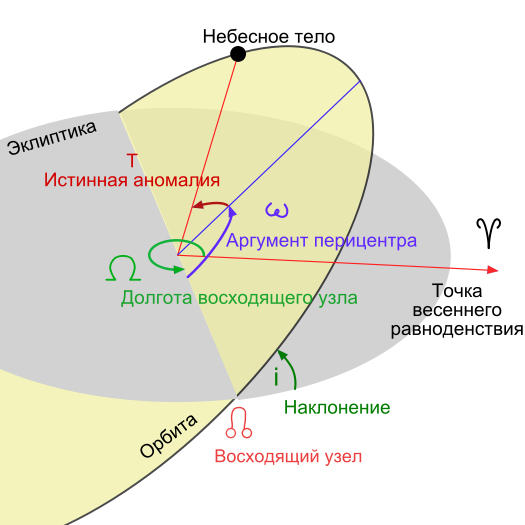
\includegraphics[scale=0.31]{525px-Orbit_ru}
\begin{figure}[h!]
\caption{Кеплеровы элементы орбиты}
\end{figure}
\end{center}
\subsection{Фазы планет и спутников}

\bfseries Фазой \mdseries планеты (cпутника) называется отношение площади освещённой  части видимого диска ко всей его площади.
Фаза считается по следующей формуле:
$$\Phi=\frac{1+\cos\phi}{2}=\cos^2\frac{\phi}{2}$$
Где $\phi$ --- \textbf{фазовый угол} --- угол между лучом света, падающим от Солнца на планету, и лучом, отразившимся от неё в сторону наблюдателя (Рис.6). Фаза изменяется от 0 до 1.
\begin{center}
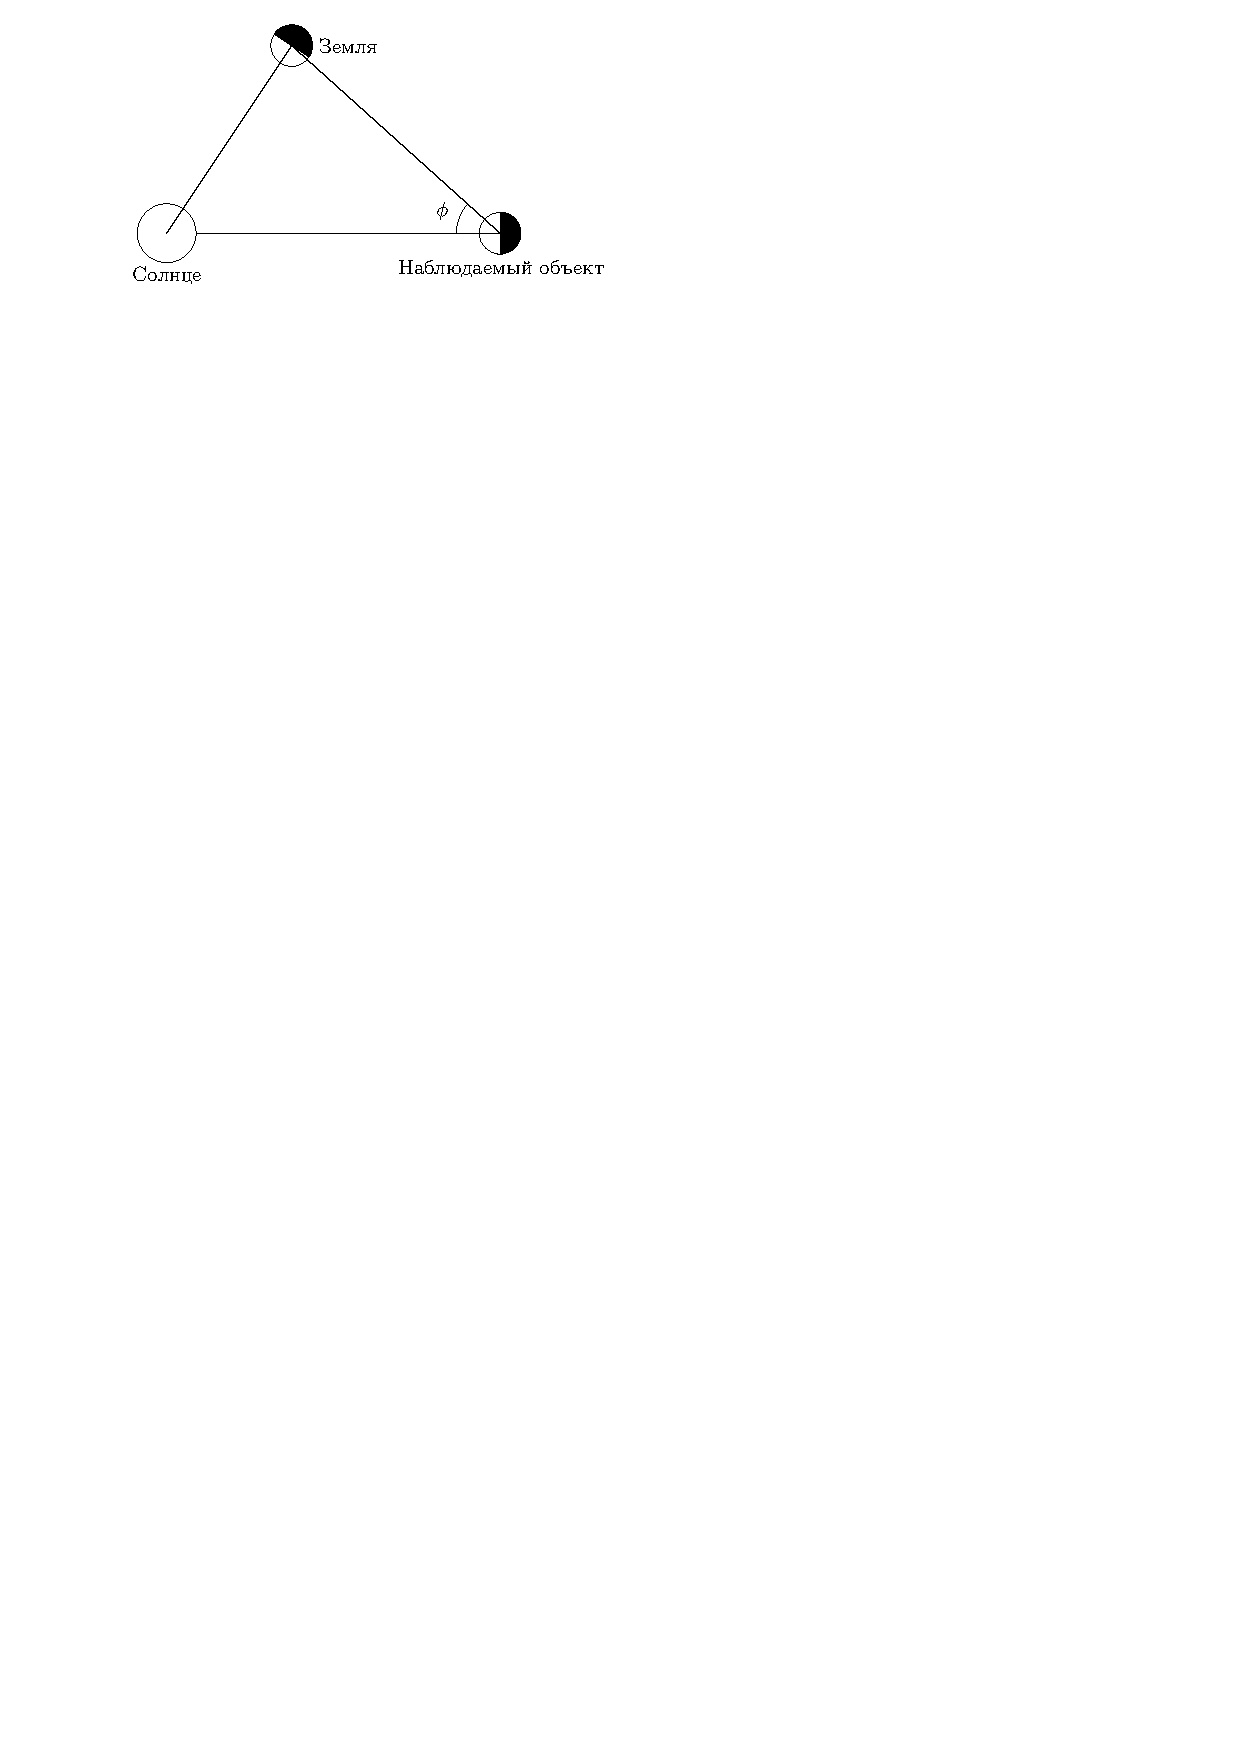
\includegraphics[width = 0.6\textwidth]{Phase_angle}
\begin{figure}[h!]
\caption{Фазовый угол}
\end{figure}
\end{center}
\subsection{Аберрация}

\textbf{Аберрация} --- явление, состоящее в том, что движущийся наблюдатель видит светило не в том направлении, в котором он видел бы его в тот же момент, если бы находился в покое. 
Угол аберрационного смещения можно найти по слейдующей формуле:
$$\sigma=\frac{v}{c}\sin\theta$$
Где $v$ --- скорость наблюдателя, $\theta$ --- угол между направлением вектора скорости наблюдателя и направлением на объект.
\subsection{Приливы и отливы}
Ускорение в центре Земли($T$) считется по слейдующей формуле: $$\omega_T=\frac{GM}{r^2}$$
Где $m$ --- масса Луны, $r^2$ --- расстояние между центрами Земли и Луны. Ускорения в точках A и B равны:
$$\omega_A=\frac{GM}{(r-R)^2} \text{ и } \omega^B=\frac{GM}{(r+R)^2}$$
Где $R$ --- радиус Земли. Ускорение точки A относительно точки T равно:
$$\omega_A-\omega_T=Gm\frac{2rR-R^2}{(r-R)^2r^2}$$
Так как $R\ll r$, то $$\omega_A-\omega_T=\frac{Gm2R}{r^3}$$

Под действием лунного притяжения водная оболочка Земли принимает форму эллипсоида, который вытянут по направлению к Луне. Близ точек $А$ и $В$ будет прилив, а у точек $F$ и $D$ --- отлив (Рис.7).
\begin{center}
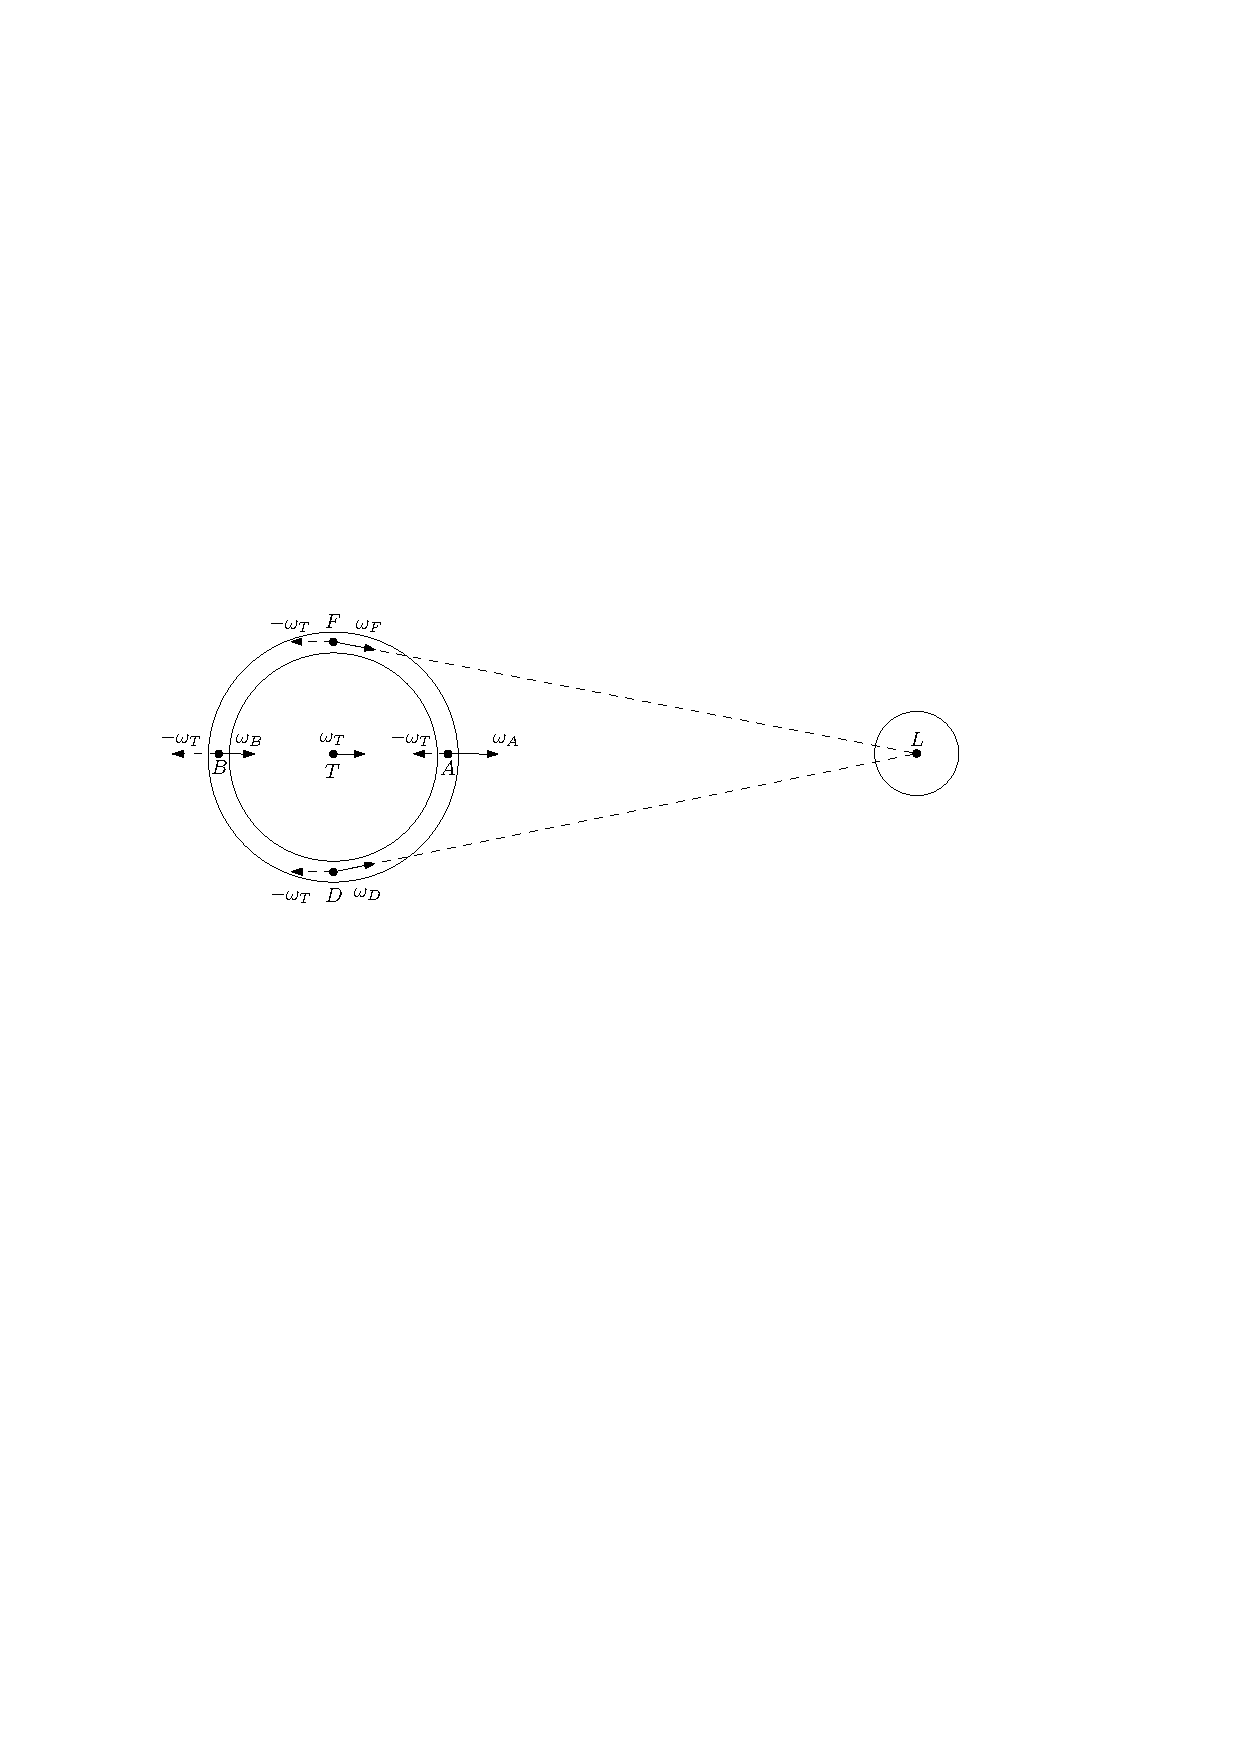
\includegraphics[width = 1\textwidth]{Ebb_and_flow}
\begin{figure}[h!]
\caption{К объяснению приливных сил}
\end{figure}
\end{center}
\subsection{Солнечные и лунные затмения. Сарос}
\subsubsection{Полное солнечное затмение}
Диаметр тени спутника при полном центральном затмении (когда центры трёх тел лежат на одной прямой), с большой точностью равен:
$$d_\text{т}=2\frac{R_\text{л}(a-R_\text{з})-R_\text{с}(a-R_\text{з})}{a-a_\text{л}}$$
Где $R_\text{л}$ --- радиус Луны, $R_\text{з}$ --- радиус Земли, $R_\text{с}$ --- радиус Солнца, $a$ --- расстояние от Земли до Солнца, $a_\text{л}$ --- расстояние от Земли до Луны.

Среднее значение  этой величины около 200 км, максимальное около 215 км. При нецентральном затмении максимальный диаметр тени Луны на поверхности Земли может достигать 270 км (Рис.8).
\begin{center}
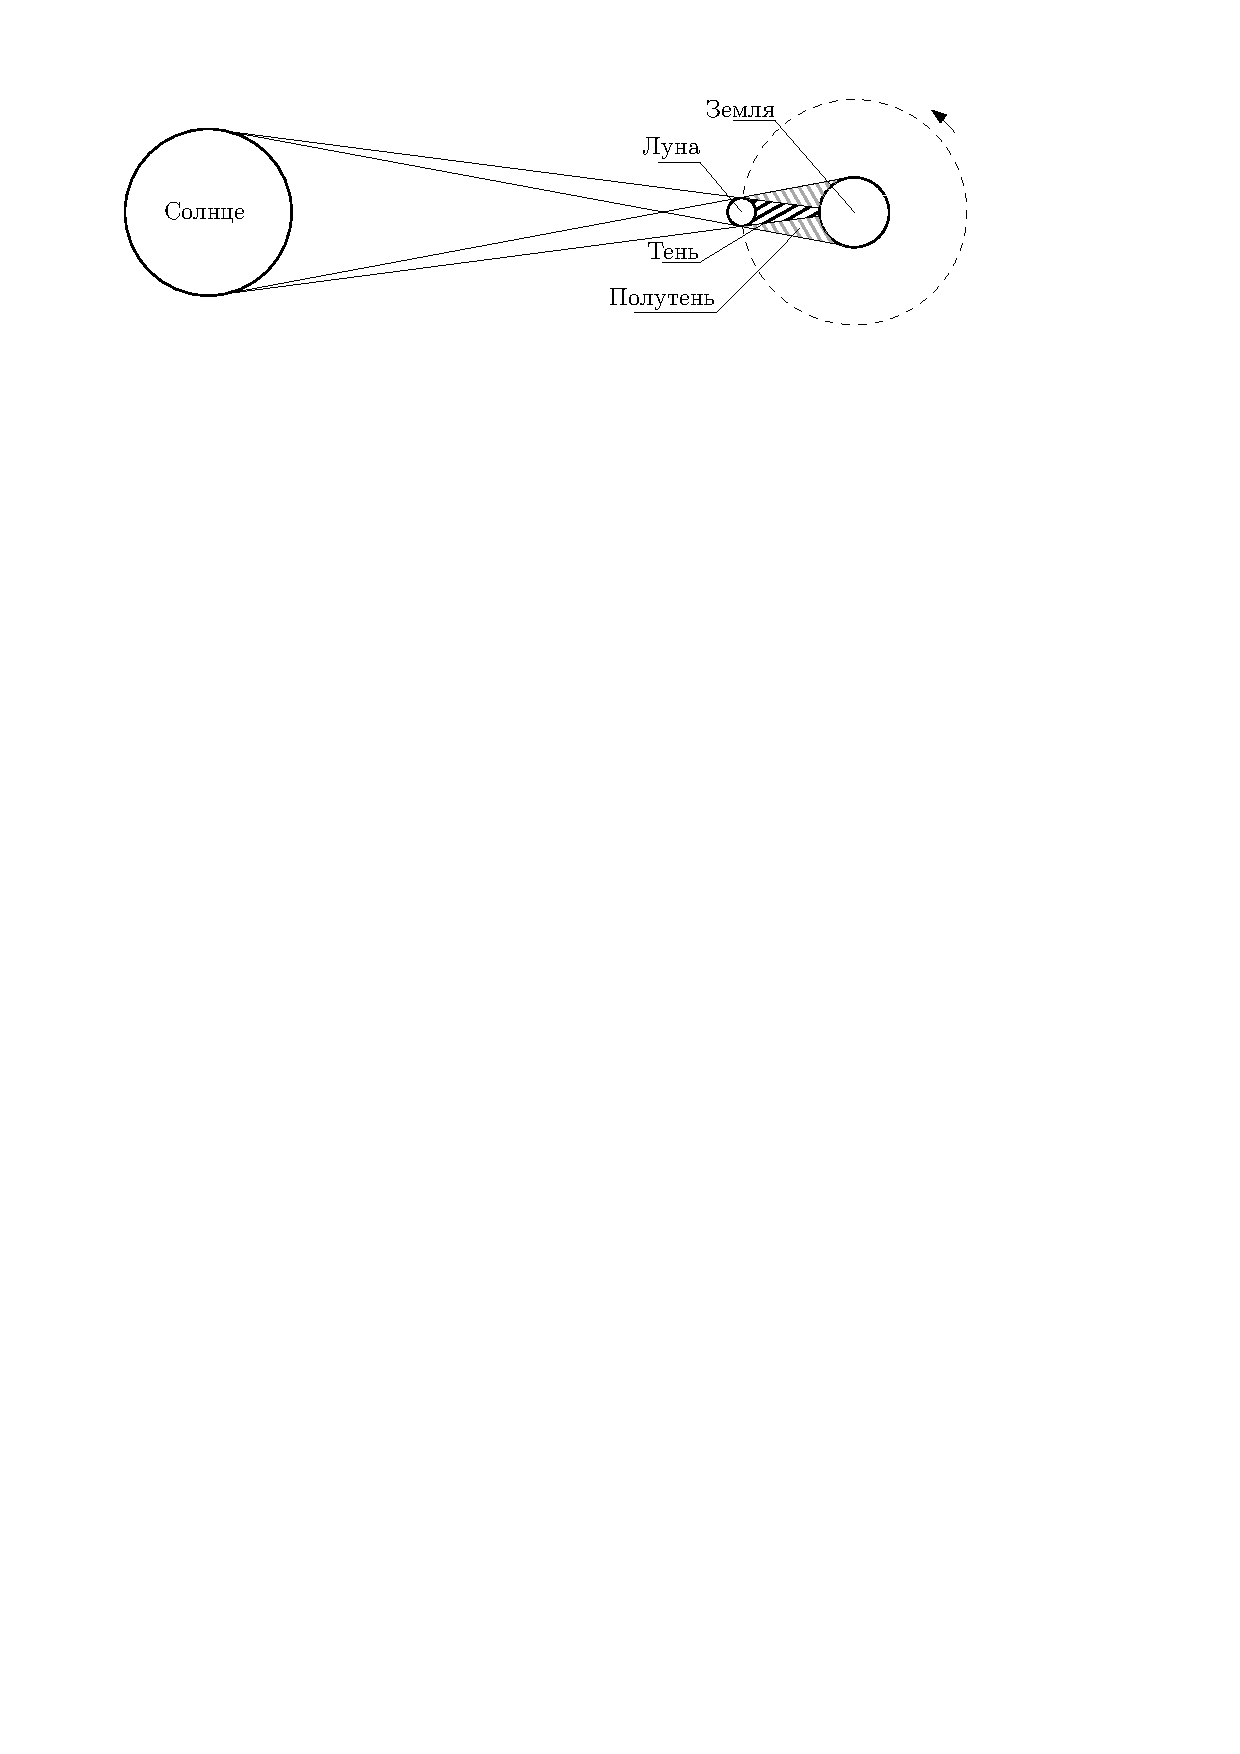
\includegraphics[width = 1.05\textwidth]{full_sollar_eclipse}
\begin{figure}[h!]
\caption{Полное солнечное затмение}
\end{figure}
\end{center}
\subsubsection{Кольцеобразное солнечное затмение}
При кольцеобразном солнечном затмении Луна относительно Земли расположена так, что конус её тени не достаёт до поверхности планеты, и вокруг Луны можно наблюдать яркое кольцо незакрытой части солнечного диска (Рис.9).
\begin{center}
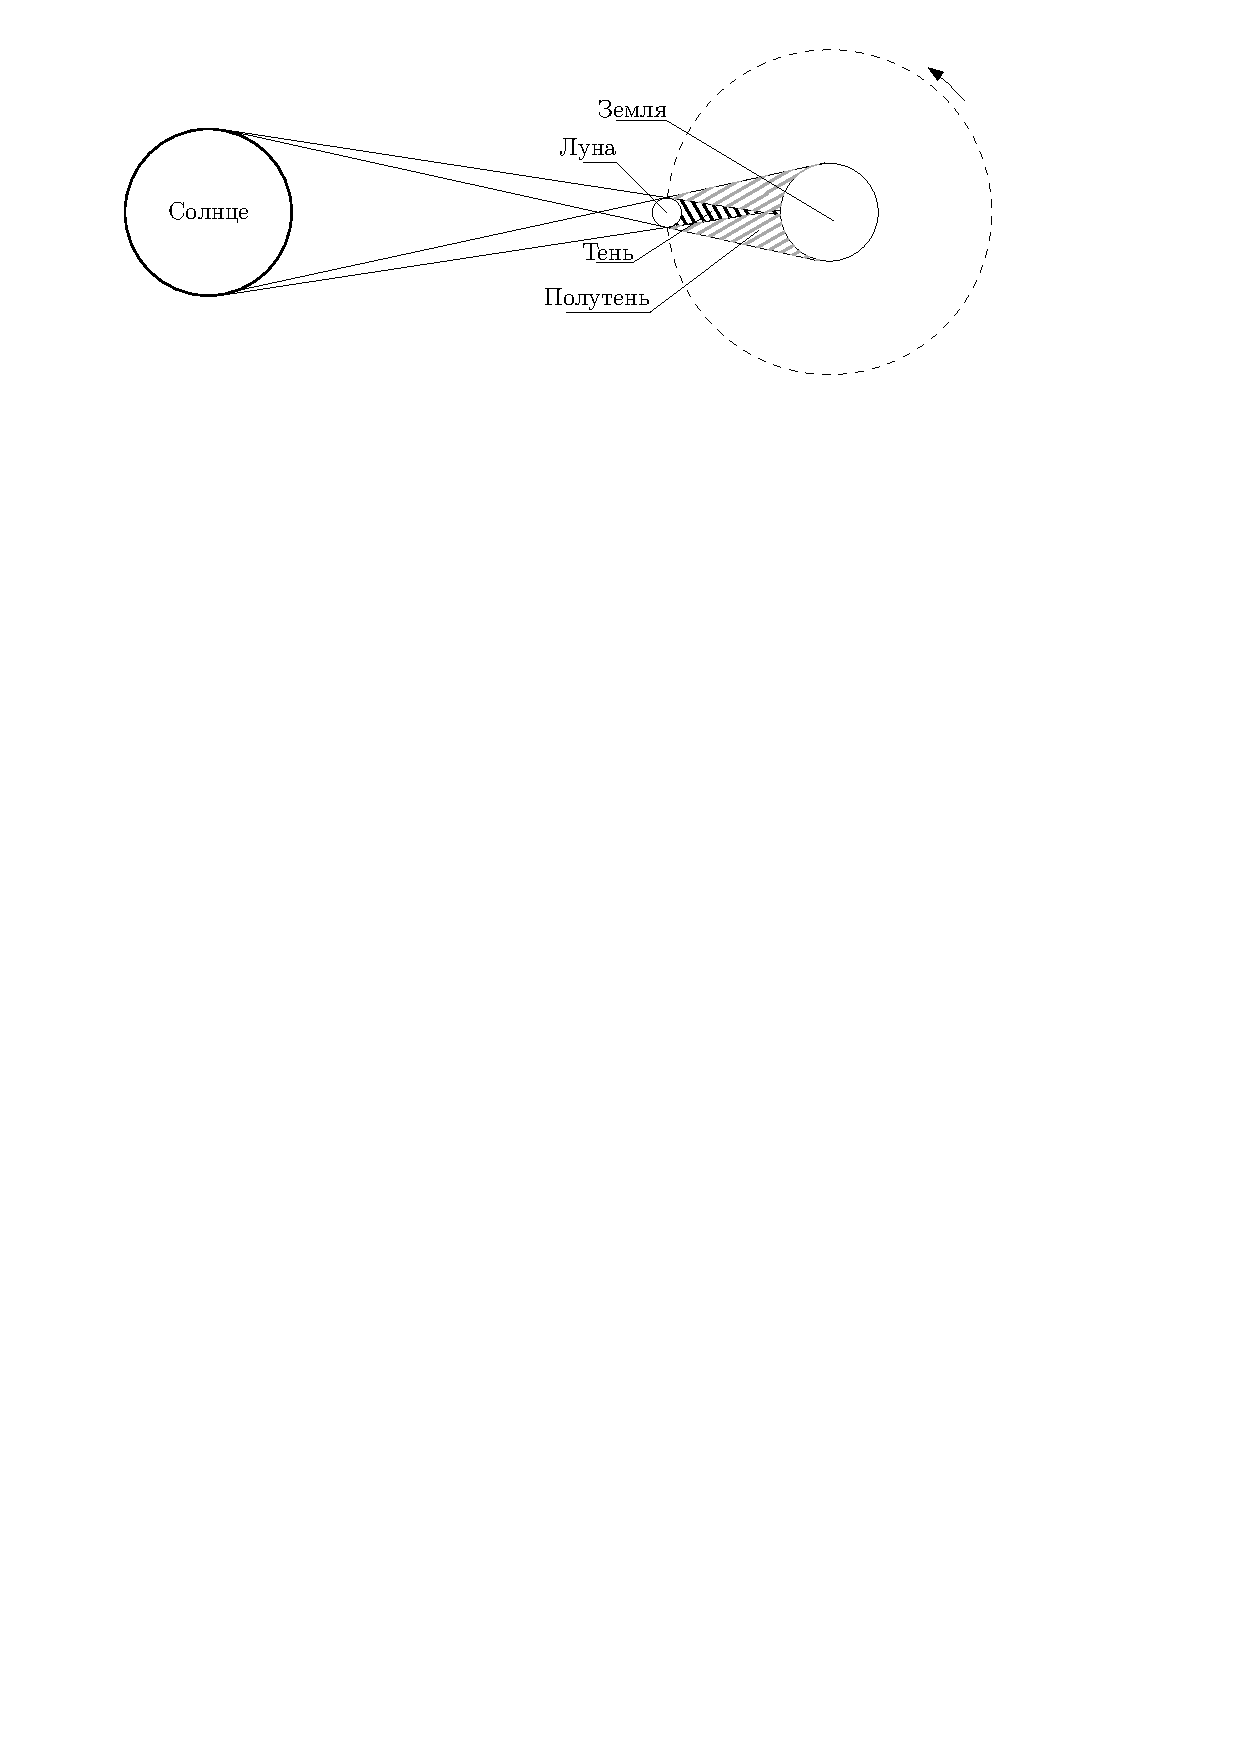
\includegraphics[width = 0.95\textwidth]{partly_sollar_eclipse}
\begin{figure}[h!]
\caption{Кольцеобразное солнечное затмение}
\end{figure}
\end{center}
\subsubsection{Лунное затмение}

Лунное затмение в отличие от солнечного, видно со всего ночного полушария. Диаметр земной тени на расстоянии Луны превышает размер последней примерно в 2.5-3 раза (Рис.10).

\textbf{Сарос} --- промежуток  времени, по прошествии которого солнечные и лунные затмения повторяются в прежнем порядке.

Этот период почти в точности равен:
\begin{enumerate}
\item 242 драконических месяца;
\item 223 синодических месяца;
\end{enumerate}

Таким образом, сарос длится примерно 18 лет 11 дней 8 часов.

\textbf{Синодический месяц} --- промежуток времени между одинаковыми фазами Луны. Он равен 29.53 суток.

\textbf{Драконический месяц} --- промежуток времени между двумя последовательными прохождениями Луны через один и тот же узел орбиты. Драконический месяц равен 27.21 суток.
\begin{center}
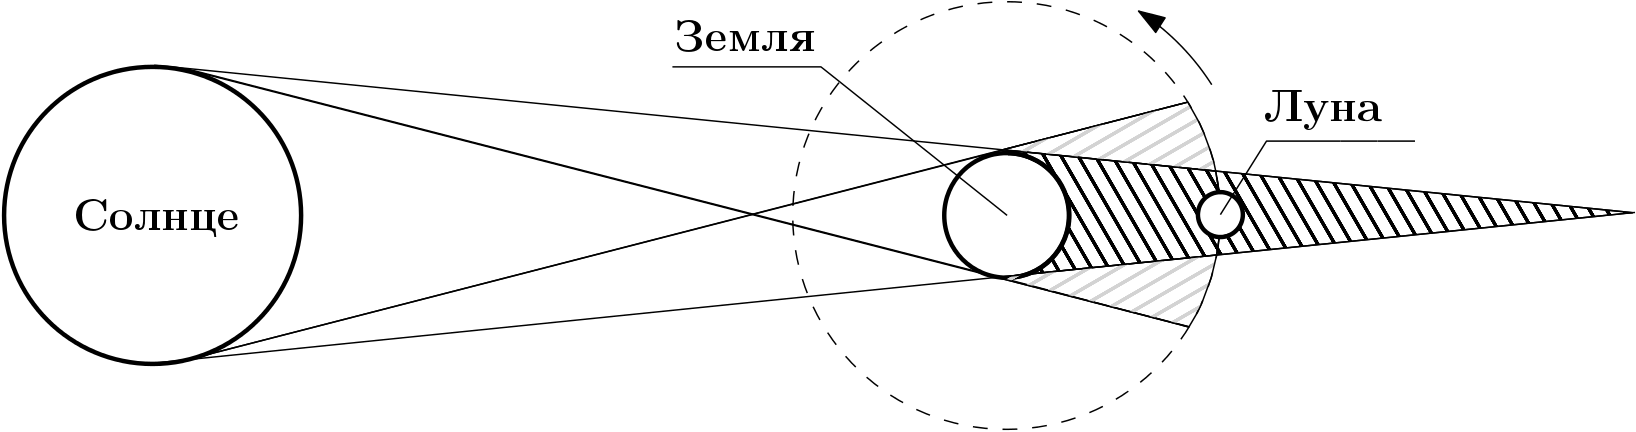
\includegraphics[scale=0.27]{moon_eclipse}
\begin{figure}[h!]
\caption{Лунное затмение}
\end{figure}
\end{center}
\subsubsection{Фаза затмения}
Очень важной характеристикой любого затмения является его фаза. \textbf{Фаза затмения} --- отношение закрытой части диаметра затмеваемого тела, проходящей через уентр затмевающего тела, к полному диаметру затмеваемого тела. Для полного затмения эта величина считается немного иначе (см. ниже). Для Луны затмевающим "телом" является тень Земли. Фазу частного и полного затмения можно вычислить по слейдующим формулам (Рис.11):
$$\Phi_{\text{ч}}=\frac{x}{D} \text{ и } \Phi_{\text{п}}=1+\frac{d}{D}$$
Где $D$ --- диаметр затмеваемого тела.
\begin{center}
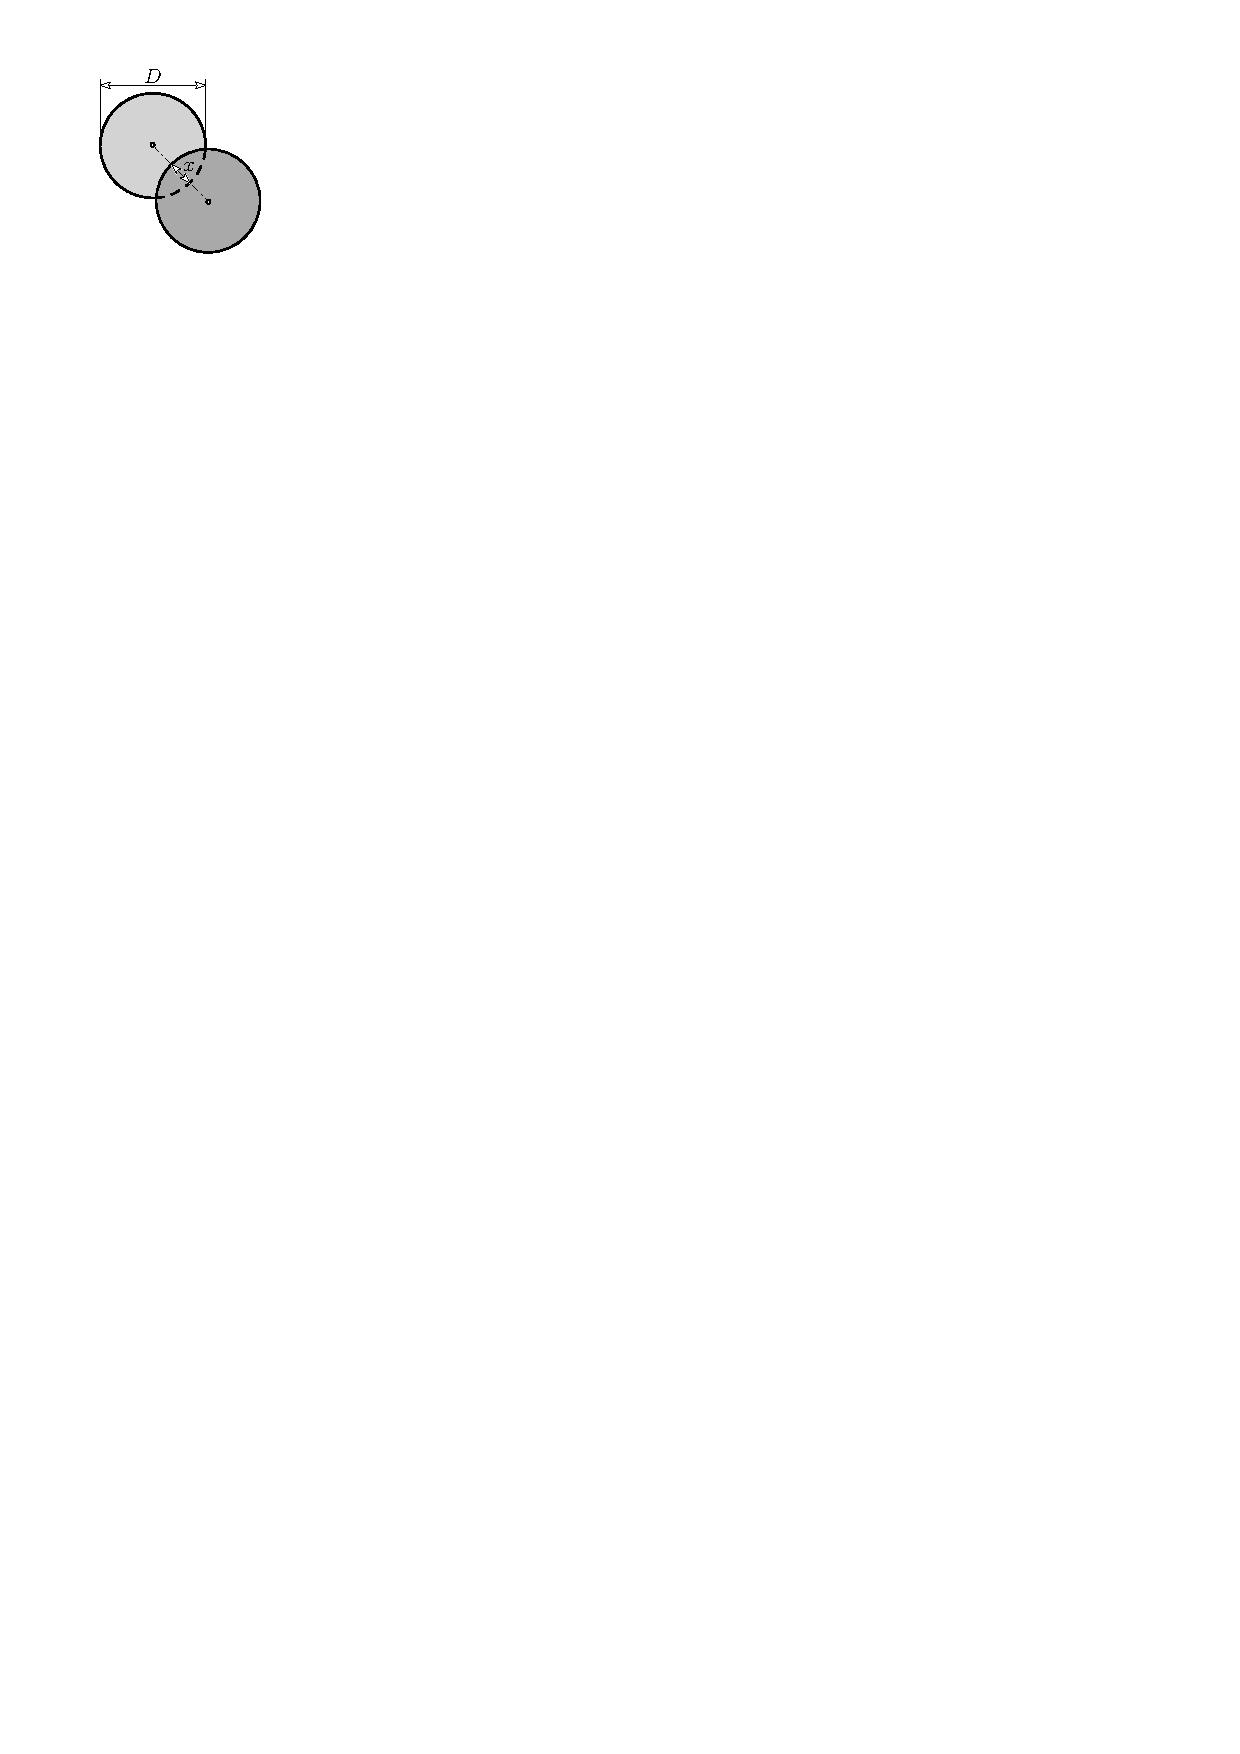
\includegraphics[width = 0.3\textwidth]{Phases}
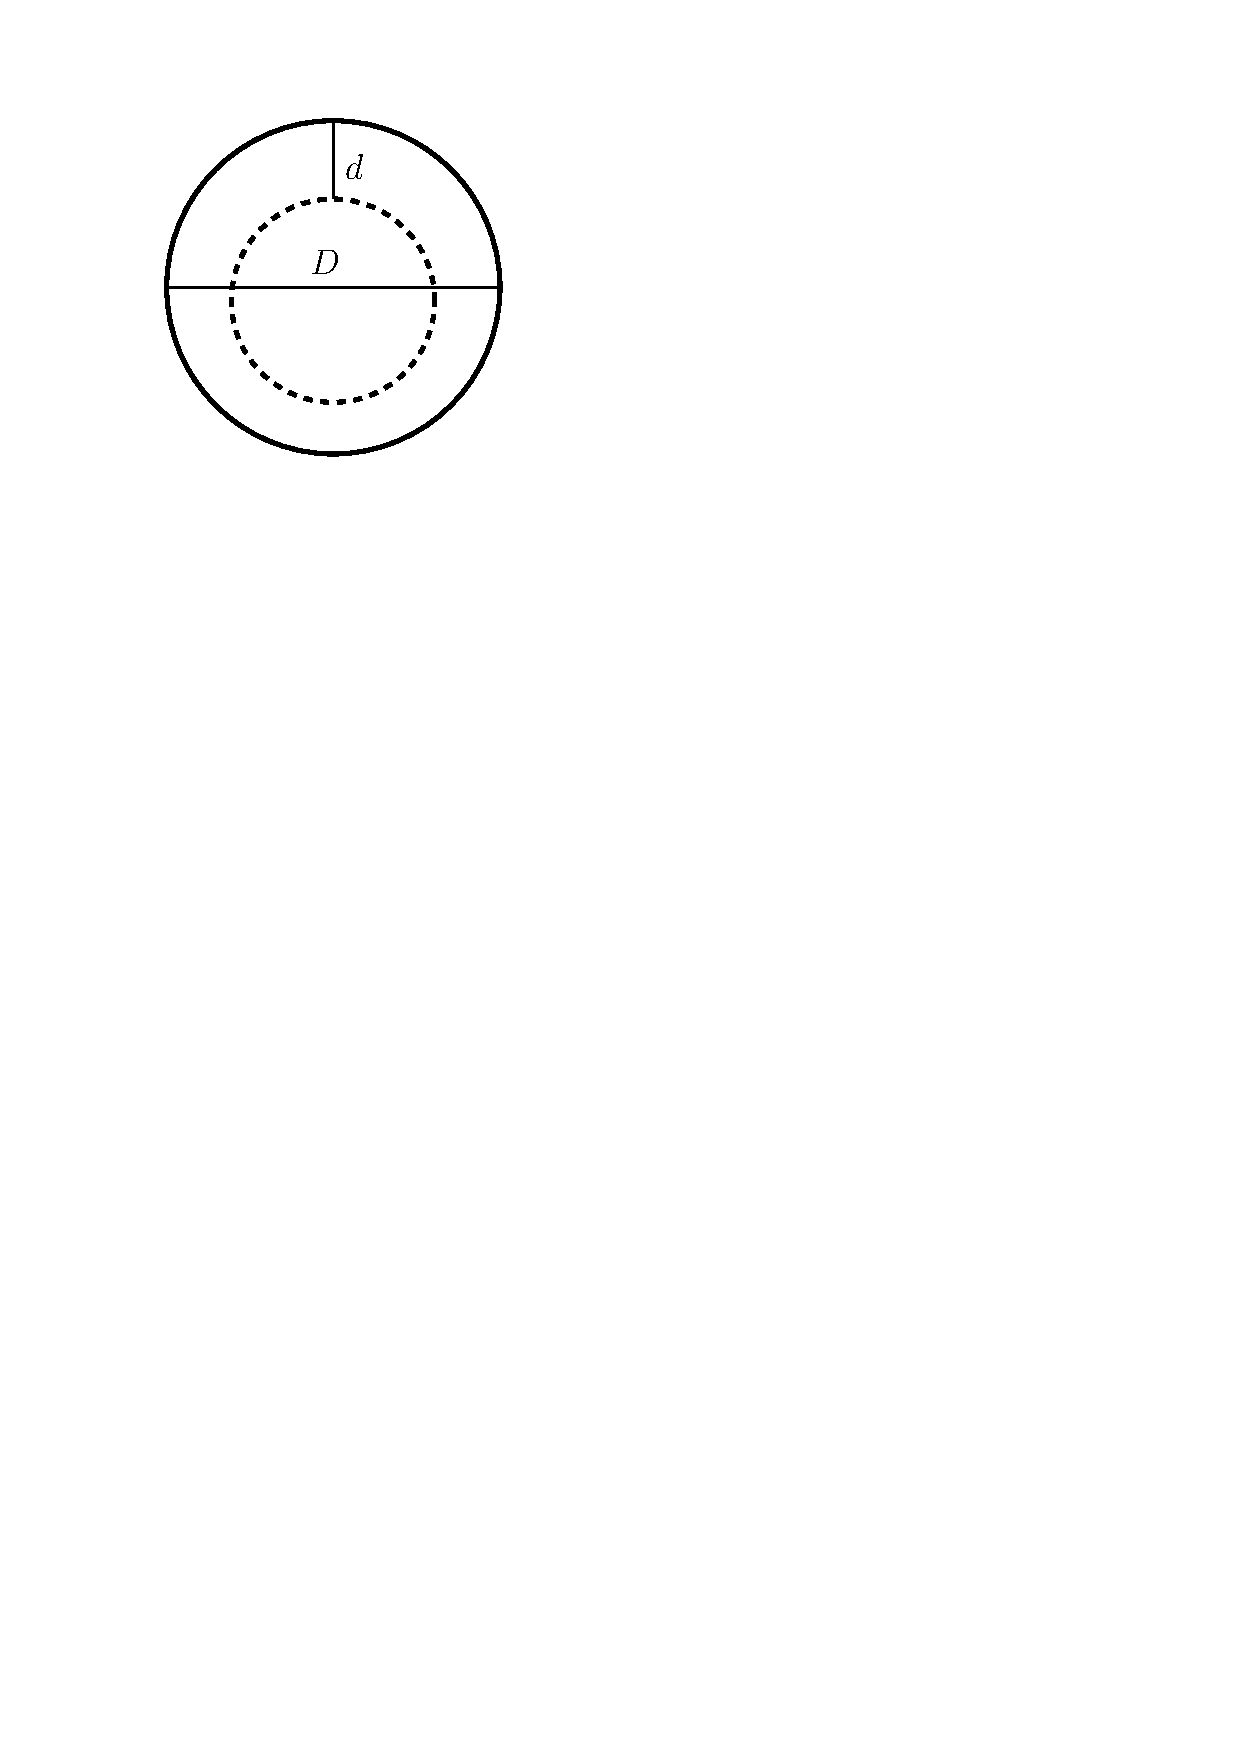
\includegraphics[width = 0.3\textwidth]{Phases_2}
\begin{figure}[h!]
\caption{Частное и полное затмение}
\end{figure}
\end{center}

Иногда вводят такое понятие, как \textbf{площадная фаза затмения}, т.е. отношение площади закрытой части диска затмеваемого диска к полоной площади его диска. Чаще площадную фазу используют применительно к двойным звёздам, когда считают падение блеска при затмении одной звезды другой.
\subsection{Прецессия}

Ось вращения Земли совершает прецессионное движение --- описывает вокруг оси эклиптики  конус радиусом основания 23.5$^\circ$ с периодом около 26 000 лет. Из-за этого меняется положение полюс мира. Например, сейчас полюс мира практически совпадает с Полярной звездой ($\alpha$ Малой Медведицы), а 15 000 лет назад роль Полярной звезды играла Вега ($\alpha$ Лиры). Если считать, что величина прецессии постоянна, то полюсы мира описывают вокруг полюсов эклиптики малые круги с радиусом 23.5$^\circ$. В действительности же величина прецессии меняется, поэтому путь полюсов мира представляет собой не окружность, а спираль.

Поворот оси Земли имеет различные последствия. Во-первых, меняется продолжительность тропического года, он становится примерно на 20 минут короче звёздного. Во-вторых, из-за прецессии меняется вид звёздного неба, хотя происходит это очень медленно (Рис.12).
\begin{center}
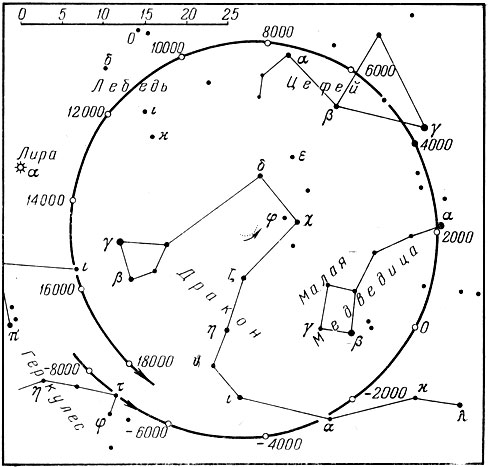
\includegraphics[scale=0.46]{000041}
\begin{figure}[h!]
\caption{Прецессионное движение северного полюса мира}
\end{figure}
\end{center}
\subsection{Точки Лагранжа}

\textbf{Точки Лагранжа} --- точки в системе из двух массивных тел, в которых третье тело с пренебрежимо малой массой, не испытывающее воздействие никаких других сил, кроме гравитационных, со стороны двух первых тел, может оставаться неподвижным относительно этих тел (Рис.13).

Точки $L_1$, $L_2$ и $L_3$ лежат на одной прямой, соединяющей два массивных тела. Точки $L_4$ и $L_5$ образуют равносторнние треугольники с массивными телами.

Приближённые формулы для вычислений расстояний до $L_1$, $L_2$ и $L_3$ от центра масс:
$$r_1=R\left(1-\sqrt[3]{\frac{\alpha}{3}}\right); r_2=R\left(1+\sqrt[3]{\frac{\alpha}{3}}\right); r_3=\left(1+\frac{5}{12}\alpha\right)$$
Где $\alpha=M_1/(M_2+M_3)$, $R$ --- расстояние между телами, $M_1$ --- масса более массивного тела, $M_2$ --- масса второго тела.

Если $M_2\ll M_1$, то точки $L_1$ и $L_2$ находятся примерно на равном расстоянии от тела $M_2$. Примерное значение этого расстояния можно вычислить по формуле:
$$r\approx R\sqrt[3]{\frac{M_2}{3M_1}}$$
\begin{center}
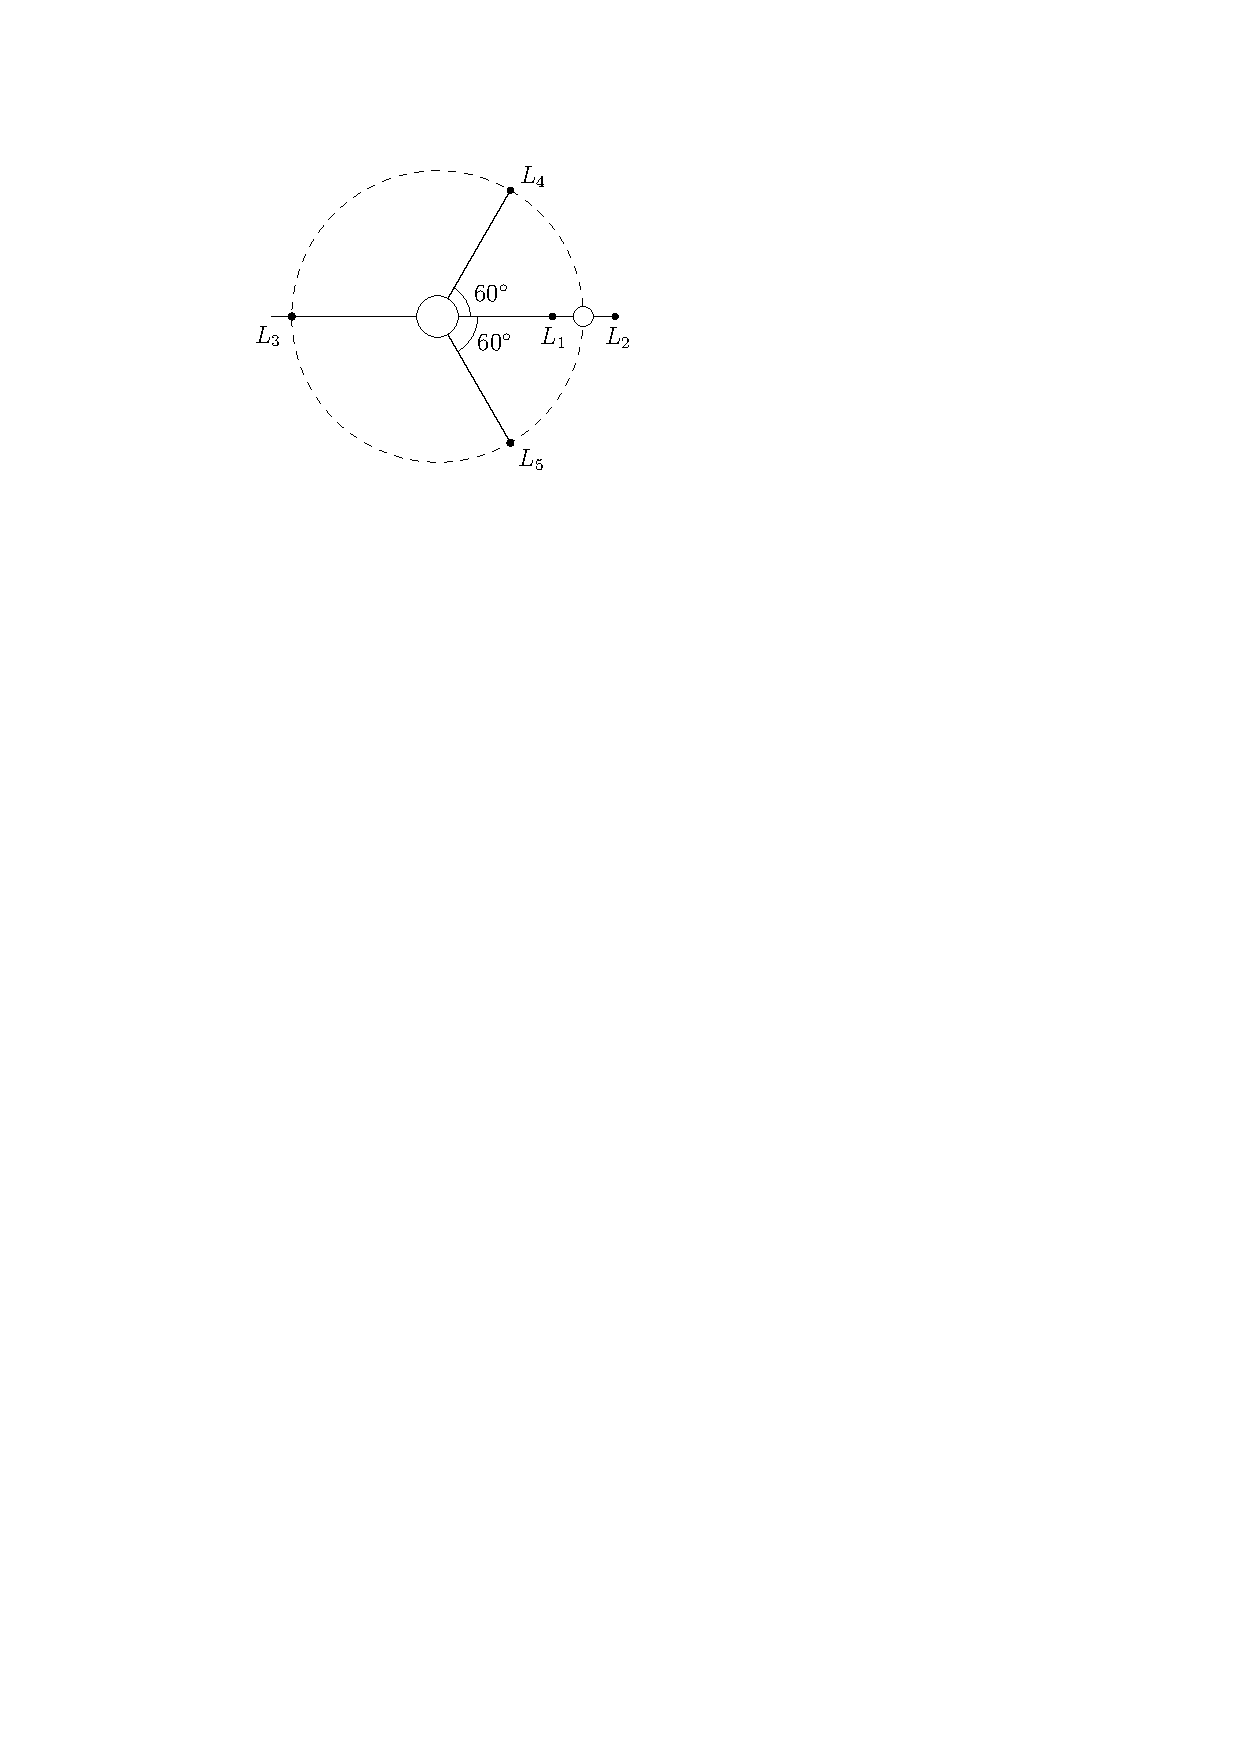
\includegraphics[width = 0.45\textwidth]{Lagrange's_points}
\begin{figure}[h!]
\caption{Точки Лагранжа}
\end{figure}
\end{center}
\subsection{Расстояние и размеры}
$$r=\frac{1}{\pi}$$
Где $r$ --- расстояние до звезды, $\pi$ --- годовой параллакс звезды.
$$r=\frac{R_{\text{З}}}{\sin p_0}=\frac{3438'}{p_0'}R_{\text{З}}=\frac{206265''}{p_0''}R_{\text{З}}$$
Где $R_{\text{З}}$ --- радиус Земли, $p_0$ --- горизонтальный экваториальный параллакс.

\textbf{Правило Тициуса-Боде} --- эмпирическая формула приблизительно описывающая радиусы орбит планет от Солнца:
$$r=\frac{n+4}{10}$$
Где $n=0, 3 ,6, 12, 24, 48...$ или
$$r=\frac{3\cdot 2^n+4}{10}$$
Где $n=-\infty, 0, 1, 2...$
$$R=r\frac{\rho'}{3238'}=r\frac{\rho''}{206265''}$$
Где $R$ --- радиус объекта, $\rho$ --- угловые размеры объекта.
\begin{center}
\section{Конические сечения}
\end{center}
\subsection{Эллипс}
\textbf{Эллипс} --- плоская замкнутая кривая, сумма расстояний от любой точки котрой до двух фиксированных точек, называемых фокусами, постоянна и равна удвоенной большой полуоси эллипса.
$$F_1M+F_2M=const=2a$$
Главные отрезки эллипса:
\begin{enumerate}
\item Большая полуось ($a$)
\item Малая полуось ($b$)
\item Фокусное расстояние ($c$)
\end{enumerate}
$a$, $b$ и $c$ связаны слейдующим образом: $b^2+c^2=a^2$, что несложно вывести из определения эллипса.
 Эксцентриситет ($e$) --- числовая характеристика, показывающая степень отклонения от окружности. В эллипсе $0<e<1$.
 \begin{center}
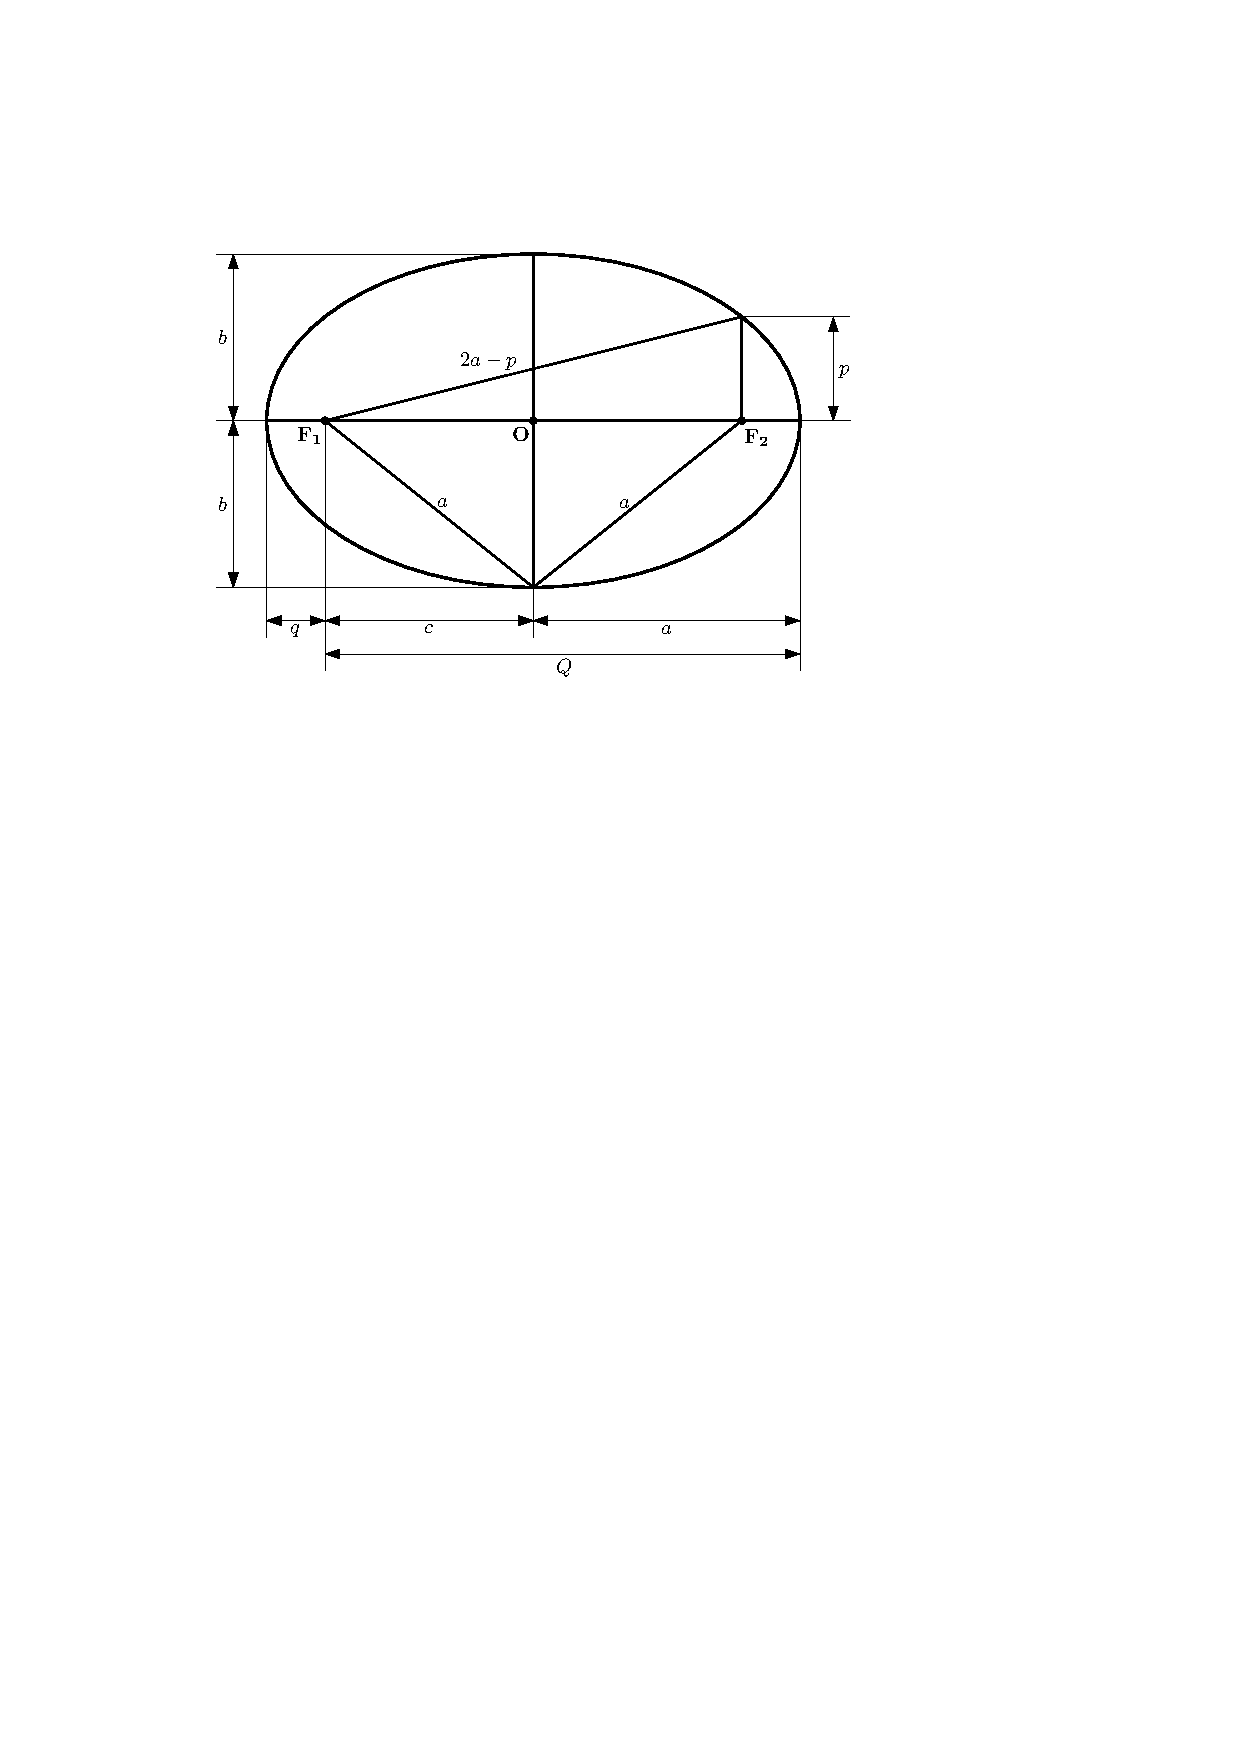
\includegraphics[width = 0.8\textwidth]{Ellips}
\begin{figure}[h!]
\caption{Эллипс}
\end{figure}
\end{center}

\end{document}